\chapter{Linked List}
% Content for Chapter 8

\section*{Introduction}
Linked lists are dynamic data structures in which nodes are linked together via pointers. They allow efficient insertions and deletions compared to static arrays. In this chapter, we cover three types of linked lists:
\begin{enumerate}
  \item \textbf{Singly Linked List}
  \item \textbf{Doubly Linked List}
  \item \textbf{Circular Linked List}
\end{enumerate}
Each type is explained in detail with corresponding C++ implementations, diagrams, and a summary of time and space complexities for common operations.

\section{Singly Linked List}

\subsection{Node Structure (Singly)}
\begin{lstlisting}[style=cppstyle, caption={Singly Linked List Node Structure in C++}]
struct Node {
    int data;
    Node* next;
    // Constructor for convenience
    Node(int val) : data(val), next(nullptr) {}
};
\end{lstlisting}

% --- Additional Theory for Singly Linked List ---
\textbf{Theory:} A singly linked list consists of nodes where each node holds data and a pointer to the next node. This design makes the list flexible in size, allowing nodes to be added or removed without reallocating or reorganizing the entire structure. However, because each node only points forward, traversing the list in reverse order is not straightforward without additional modifications.

\subsection{Operations on Singly Linked List}
\subsubsection{Insertion}
\begin{lstlisting}[style=cppstyle, caption={Insert at Front in Singly Linked List}]
void insertAtFront(Node*& head, int val) {
    Node* newNode = new Node(val);
    newNode->next = head;
    head = newNode;
}
\end{lstlisting}

\begin{lstlisting}[style=cppstyle, caption={Insert at End in Singly Linked List}]
void insertAtEnd(Node*& head, int val) {
    Node* newNode = new Node(val);
    if (!head) {
        head = newNode;
        return;
    }
    Node* temp = head;
    while (temp->next)
        temp = temp->next;
    temp->next = newNode;
}
\end{lstlisting}

\begin{lstlisting}[style=cppstyle, caption={Insert at Position in Singly Linked List}]
void insertAtPosition(Node*& head, int pos, int val) {
    if (pos == 0) {
        insertAtFront(head, val);
        return;
    }
    Node* newNode = new Node(val);
    Node* temp = head;
    for (int i = 0; temp != nullptr && i < pos - 1; i++)
        temp = temp->next;
    if (!temp) return; // Position out of bounds
    newNode->next = temp->next;
    temp->next = newNode;
}
\end{lstlisting}

% --- Additional Theory for Insertion in Singly Linked List ---
\textbf{Insertion Theory:} Insertion at the front of a singly linked list is very efficient (\(O(1)\)) because it simply involves updating the head pointer. Insertion at the end requires traversal of the entire list, resulting in \(O(n)\) time complexity. When inserting at a given position, the list must be traversed until that position is reached, making it \(O(n)\) as well. These operations illustrate the trade-off between flexibility and direct access in linked lists.

\subsubsection{Deletion}
\begin{lstlisting}[style=cppstyle, caption={Delete from Front in Singly Linked List}]
void deleteFromFront(Node*& head) {
    if (!head) return;
    Node* temp = head;
    head = head->next;
    delete temp;
}
\end{lstlisting}

\begin{lstlisting}[style=cppstyle, caption={Delete from End in Singly Linked List}]
void deleteFromEnd(Node*& head) {
    if (!head) return;
    if (!head->next) {
        delete head;
        head = nullptr;
        return;
    }
    Node* temp = head;
    while (temp->next && temp->next->next)
        temp = temp->next;
    delete temp->next;
    temp->next = nullptr;
}
\end{lstlisting}

\begin{lstlisting}[style=cppstyle, caption={Delete from Position in Singly Linked List}]
void deleteAtPosition(Node*& head, int pos) {
    if (!head) return;
    if (pos == 0) {
        deleteFromFront(head);
        return;
    }
    Node* temp = head;
    for (int i = 0; temp != nullptr && i < pos - 1; i++)
        temp = temp->next;
    if (!temp || !temp->next) return; // Position out of bounds
    Node* delNode = temp->next;
    temp->next = delNode->next;
    delete delNode;
}
\end{lstlisting}

% --- Additional Theory for Deletion in Singly Linked List ---
\textbf{Deletion Theory:} Deletion operations in a singly linked list are efficient if the node to be deleted is known (\(O(1)\)). However, if a search is needed to find the node, the operation becomes \(O(n)\). The simplicity of pointer adjustments in deletion is a key advantage over array-based structures.

\subsubsection{Search}
\begin{lstlisting}[style=cppstyle, caption={Search in Singly Linked List}]
int search(Node* head, int key) {
    int index = 0;
    while (head) {
        if (head->data == key)
            return index;
        head = head->next;
        index++;
    }
    return -1; // Not found
}
\end{lstlisting}

% --- Additional Theory for Search in Singly Linked List ---
\textbf{Search Theory:} Since singly linked lists are sequential, searching for an element requires traversing the list from the head until the element is found, leading to \(O(n)\) time complexity. This is less efficient compared to direct indexing in arrays but is acceptable given the dynamic nature of linked lists.

\subsection{Diagram: Singly Linked List}
\begin{center}
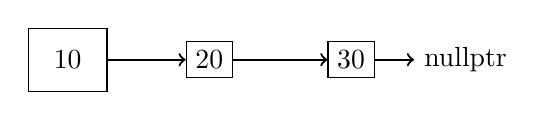
\begin{tikzpicture}[node distance=1.8cm, auto]
  \node (n1) [draw, rectangle, minimum width=1cm, minimum height=0.8cm] {10};
  \node (n2) [draw, rectangle, right of=n1] {20};
  \node (n3) [draw, rectangle, right of=n2] {30};
  \draw[->, thick] (n1.east) -- (n2.west);
  \draw[->, thick] (n2.east) -- (n3.west);
  \draw[->, thick] (n3.east) -- ++(0.5,0) node[right]{nullptr};
\end{tikzpicture}
\captionof{figure}{Singly Linked List Diagram}
\end{center}

\newpage

\section{Doubly Linked List}

\subsection{Node Structure (Doubly)}
\begin{lstlisting}[style=cppstyle, caption={Doubly Linked List Node Structure in C++}]
struct DNode {
    int data;
    DNode* next;
    DNode* prev;
    DNode(int val) : data(val), next(nullptr), prev(nullptr) {}
};
\end{lstlisting}

\subsection{Operations on Doubly Linked List}
\subsubsection{Insertion}
\begin{lstlisting}[style=cppstyle, caption={Insert at Front in Doubly Linked List}]
void insertAtFront(DNode*& head, int val) {
    DNode* newNode = new DNode(val);
    newNode->next = head;
    if (head)
        head->prev = newNode;
    head = newNode;
}
\end{lstlisting}

\begin{lstlisting}[style=cppstyle, caption={Insert at End in Doubly Linked List}]
void insertAtEnd(DNode*& head, int val) {
    DNode* newNode = new DNode(val);
    if (!head) {
        head = newNode;
        return;
    }
    DNode* temp = head;
    while (temp->next)
        temp = temp->next;
    temp->next = newNode;
    newNode->prev = temp;
}
\end{lstlisting}

% --- Additional Theory for Doubly Linked List Insertion ---
\textbf{Theory:} Doubly linked lists maintain two pointers in each node, which allows traversal in both directions. This feature simplifies certain operations like deletion and backward traversal but requires additional memory for the extra pointer.

\subsubsection{Deletion}
\begin{lstlisting}[style=cppstyle, caption={Delete from Front in Doubly Linked List}]
void deleteFromFront(DNode*& head) {
    if (!head) return;
    DNode* temp = head;
    head = head->next;
    if (head)
        head->prev = nullptr;
    delete temp;
}
\end{lstlisting}

\begin{lstlisting}[style=cppstyle, caption={Delete from End in Doubly Linked List}]
void deleteFromEnd(DNode*& head) {
    if (!head) return;
    if (!head->next) {
        delete head;
        head = nullptr;
        return;
    }
    DNode* temp = head;
    while (temp->next)
        temp = temp->next;
    temp->prev->next = nullptr;
    delete temp;
}
\end{lstlisting}

\begin{lstlisting}[style=cppstyle, caption={Search in Doubly Linked List}]
int search(DNode* head, int key) {
    int index = 0;
    while (head) {
        if (head->data == key)
            return index;
        head = head->next;
        index++;
    }
    return -1;
}
\end{lstlisting}

\subsection{Diagram: Doubly Linked List}
\begin{center}
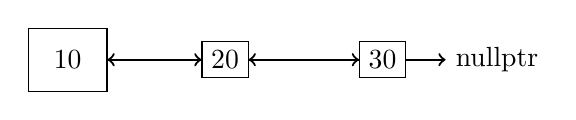
\begin{tikzpicture}[node distance=2cm, auto]
  \node (d1) [draw, rectangle, minimum width=1cm, minimum height=0.8cm] {10};
  \node (d2) [draw, rectangle, right of=d1] {20};
  \node (d3) [draw, rectangle, right of=d2] {30};
  \draw[->, thick] (d1.east) -- (d2.west);
  \draw[->, thick] (d2.west) -- (d1.east);
  \draw[->, thick] (d2.east) -- (d3.west);
  \draw[->, thick] (d3.west) -- (d2.east);
  \draw[->, thick] (d3.east) -- ++(0.5,0) node[right]{nullptr};
\end{tikzpicture}
\captionof{figure}{Doubly Linked List Diagram}
\end{center}

\newpage

\section{Circular Linked List}

\subsection{Node Structure (Circular)}
\begin{lstlisting}[style=cppstyle, caption={Circular Linked List Node Structure in C++}]
struct CNode {
    int data;
    CNode* next;
    CNode(int val) : data(val), next(nullptr) {}
};
\end{lstlisting}

\subsection{Operations on Circular Linked List}
\subsubsection{Insertion}
\begin{lstlisting}[style=cppstyle, caption={Insert in Circular Linked List}]
void insertCircular(CNode*& head, int val) {
    CNode* newNode = new CNode(val);
    if (!head) {
        head = newNode;
        newNode->next = head;
        return;
    }
    CNode* temp = head;
    while (temp->next != head)
        temp = temp->next;
    temp->next = newNode;
    newNode->next = head;
}
\end{lstlisting}

\subsubsection{Deletion}
\begin{lstlisting}[style=cppstyle, caption={Delete Node in Circular Linked List}]
void deleteCircular(CNode*& head, int key) {
    if (!head) return;
    // If head is to be deleted
    if (head->data == key) {
        if (head->next == head) { // Only one node exists
            delete head;
            head = nullptr;
            return;
        }
        // Find last node to update its next pointer
        CNode* temp = head;
        while (temp->next != head)
            temp = temp->next;
        CNode* del = head;
        head = head->next;
        temp->next = head;
        delete del;
        return;
    }
    // Delete node other than head
    CNode* curr = head;
    while (curr->next != head && curr->next->data != key)
        curr = curr->next;
    if (curr->next->data == key) {
        CNode* del = curr->next;
        curr->next = del->next;
        delete del;
    }
}
\end{lstlisting}

\subsubsection{Search}
\begin{lstlisting}[style=cppstyle, caption={Search in Circular Linked List}]
int searchCircular(CNode* head, int key) {
    if (!head) return -1;
    int index = 0;
    CNode* temp = head;
    do {
        if (temp->data == key)
            return index;
        temp = temp->next;
        index++;
    } while (temp != head);
    return -1;
}
\end{lstlisting}

\subsection{Diagram: Circular Linked List}
\begin{center}
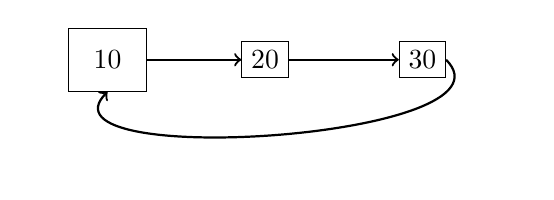
\begin{tikzpicture}[node distance=2cm, auto]
  \node (c1) [draw, rectangle, minimum width=1cm, minimum height=0.8cm] {10};
  \node (c2) [draw, rectangle, right of=c1] {20};
  \node (c3) [draw, rectangle, right of=c2] {30};
  \draw[->, thick] (c1.east) -- (c2.west);
  \draw[->, thick] (c2.east) -- (c3.west);
  \draw[->, thick] (c3.east) .. controls +(1,-1) and +(-1,-1) .. (c1.south);
\end{tikzpicture}
\captionof{figure}{Circular Linked List Diagram}
\end{center}

\section{Complexity Analysis for Linked List Operations}
\begin{table}[H]
\centering
\renewcommand{\arraystretch}{1.5}
\begin{tabular}{|l|c|c|}
\hline
\textbf{Operation} & \textbf{Time Complexity} & \textbf{Space Complexity} \\ \hline
Access             & \(O(n)\)  & \(O(n)\) (node overhead) \\ \hline
Search             & \(O(n)\)  & \(O(1)\) \\ \hline
Insertion (given pointer) & \(O(1)\) & \(O(1)\) \\ \hline
Insertion (search required) & \(O(n)\) & \(O(1)\) \\ \hline
Deletion (given pointer) & \(O(1)\) & \(O(1)\) \\ \hline
Deletion (search required) & \(O(n)\) & \(O(1)\) \\ \hline
\end{tabular}
\caption{Time and Space Complexity of Linked List Operations}
\end{table}

\section{Syntax Summary for Linked List Node Structures}
\begin{center}
\renewcommand{\arraystretch}{1.5}
\begin{tabular}{|l|l|}
\hline
\textbf{Type} & \textbf{Node Structure Syntax} \\\hline
Singly Linked List & \texttt{struct Node \{ int data; Node* next; \}} \\\hline
Doubly Linked List & \texttt{struct DNode \{ int data; DNode* next; DNode* prev; \}} \\\hline
Circular Linked List & \texttt{struct CNode \{ int data; CNode* next; \}} \\\hline
\end{tabular}
\captionof{table}{Node Structure Syntax for Different Linked Lists}
\end{center}

\section{Additional Theoretical Concepts}

\subsection{Singly Linked List Theory}
Singly linked lists are one of the simplest forms of linked lists. They are ideal for implementations where only forward traversal is needed. Their simplicity, however, comes at a cost: operations like finding the previous node require traversing the list from the head, which can be inefficient. They are best used in scenarios where memory reallocation is frequent and operations mostly involve adding or removing nodes at the head.

\subsection{Doubly Linked List Theory}
Doubly linked lists enhance singly linked lists by providing backward pointers. This allows efficient bidirectional traversal, which simplifies operations like deletion from the end or inserting before a given node. However, this comes at the cost of additional memory for the extra pointer, and the operations are slightly more complex because both pointers must be updated during insertions and deletions.

\subsection{Circular Linked List Theory}
Circular linked lists differ from the other types in that the last node points back to the first node, forming a continuous loop. This structure is useful for applications where the list needs to be traversed cyclically (e.g., round-robin scheduling). They eliminate the need for null checks at the end of the list, but careful handling is required during insertion and deletion to avoid infinite loops.

\subsection{Memory Management and Pointer Usage}
Linked lists dynamically allocate memory for each node, which means memory is used only as needed. However, the overhead of storing pointers in each node can be significant compared to array elements. In systems with limited memory, the trade-off between flexibility and memory overhead must be considered. Garbage collection (in languages that support it) or manual memory management in C++ is essential to avoid memory leaks.

\section{Conclusion}
Linked lists are versatile and powerful dynamic data structures that provide efficient insertion and deletion operations. Each type—singly, doubly, and circular—has its own advantages and trade-offs. Singly linked lists are simple and efficient for forward traversal; doubly linked lists allow for bidirectional movement; and circular linked lists facilitate continuous looping without explicit null termination. Understanding the underlying theory, along with the syntax and complexity of various operations, is crucial for designing efficient data structures and algorithms.

\vspace{1em}
This chapter provides both practical C++ implementations and theoretical insights to help you master linked list concepts.
